
\documentclass[12pt]{report}

\setlength{\oddsidemargin}{0.0in}
\setlength{\textwidth}{6.5in}
%\setlength{\topmargin}{0in}
%\setlength{\textheight}{7.5in}
\usepackage{amssymb}
\usepackage{amsfonts}
\usepackage{amsmath}
\usepackage{latexsym}
\usepackage{epsfig}

\linespread{1.1}

\newenvironment{proof}{\noindent \textbf{Proof:}}{$\Box$}
\newenvironment{claim}{\noindent \textbf{Claim:}}{}
\newenvironment{theorem}{\noindent \textbf{Theorem:}}{}
\newcommand{\infint}{\int_{-\infty}^\infty}
\newcommand{\intunit}{\int_{-1}^1}

\title{PCGSL: Playing Card Game Simulation Language}

\date{
\ \\
COMS W4115
\\
Programming Languages and Translators
\\
\today
}

\author{
Enrique Henestroza
\\
{\tt eh2348@columbia.edu}
\and
Yuriy Kagan
\\
{\tt yk2159@columbia.edu}
\and
Andrew Shu
\\
{\tt ans2120@columbia.edu}
\and
Peter Tsonev
\\
{\tt pvt2101@columbia.edu}
}

\begin{document}

\begin{titlepage}

\maketitle

\end{titlepage}

\setcounter{tocdepth}{2}

\tableofcontents

\pagebreak

\chapter{Introduction}

The Playing Card Game Simulation Language (PCGSL) is designed to be a simple programming language for programming card games. Our language allows a programmer to work within a standard set of conventions and procedures for playing card games, without having to write a large amount of code as one would have to in a general-purpose language. This allows the programmer to focus on creating randomized simulations of popular games or hands, as well as quick mock-ups of new games based around standard 52-card decks.

\section{Simple}

PCGSL is simple to learn. Using well known C-style imperative syntax conventions, our language...

\chapter{Language Tutorial}

\chapter{Language Manual}

\section{Lexical Conventions}
This section covers the lexical conventions including comments and tokens. A token is a series of contiguous characters that the compiler treats as a unit. Blanks, tabs, newlines, and comments are collectively known as �white space.� White space is ignored except as it serves to separate tokens. Some white space is required to separate otherwise adjacent identifiers, keywords, and constants. If the input stream has been parsed into tokens up to a given character, the next token is taken to include the longest string of characters that could possibly constitute a token.

\subsection{Comments}
The // characters introduce a comment; a newline terminates a comment. The // characters do not indicate a comment when occurring within a string literal. Comments do not nest. Once the // introducing a comment are seen, all other characters are ignored until the ending newline is encountered.

\subsection{Identifiers}
An identifier is a sequence of letters, digits, and underscores (\_). The first character cannot be a digit. Uppercase and lowercase letters are distinct. Identifier length is unlimited.

\subsection{Keywords}
The identifiers listed below are reserved for use as keywords and cannot be used for any other purpose. Among these are a group of reserved identifiers corresponds to card names for a standard 52-card deck.

\ \\

\noindent break  Play  CardEntities return  else Start false true Globals while If WinCondition Include var null H2	H3	H4	H5	H6	H7	H8	H9	H10	HJ	HQ	HK	HA
D2	D3	D4	D5	D6	D7	D8	D9	D10	DJ	DQ	DK	DA
C2	C3	C4	C5	C6	C7	C8	C9	C10	CJ	CQ	CK	CA
S2	S3	S4	S5	S6	S7	S8	S9	S10	SJ	SQ	SK	SA
	
\subsection{Constants}
The two types of constants are integer and character string. 

\subsubsection{Integer Constants}
An integer constant consists of a sequence of one or more digits, and is always considered decimal.

\subsubsection{String Constants}
A string constant is a sequence of characters surrounded by double quotation marks, such as �Hello World!�. We consider characters to be ASCII printable characters.

\subsection{Operators}
An operator specifies an operation to be performed. The operators are shown below: \\

\noindent $<$$-$ \ \ \ \ \
$+$$+$ \ \ \ \ \
$+$ \ \ \ \ \
$--$ \ \ \ \ \
$-$ \ \ \ \ \
$*$ \ \ \ \ \
$/$ \ \ \ \ \
$+$$=$ \ \ \ \ \
$-$$=$ \ \ \ \ \
$*$$=$ \ \ \ \ \
$/$$=$ \ \ \ \ \
$=$$=$  \ \ \ \ \
$=$ \ \ \ \ \
!$=$ \ \ \ \ \
$<$ \ \ \ \ \
$<$$=$ \ \ \ \ \	
$>$ \ \ \ \ \
$>$$=$ \ \ \ \ \	
\&\& \ \ \ \ \
$|$$|$ \ \ \ \ \
::  \ \ \ \ \
$|$  \ \ \ \ \
\~{}  \ \ \ \ \
$\hat{}$  \ \ \ \ \
$@$  \ \ \ \ \
\#  \ \ \ \ \
\textdollar  \ \ \ \ \
$>$$>$  \ \ \ \ \
$<$$<$

\subsection{Meaning of Identifiers}

Identifiers are disambiguated by their type, scope, and namespace. No identifier will have linkage, and storage duration will be determined by the scope, e.g. identifiers within the same scope will have the same storage duration.

\subsubsection{Type}
Our language has four fundamental object types � int, string, boolean, and Card. In addition, there are two derived types: list and CardEntity. There is no notion of a floating point number since it is not really needed in card games. There is also no need for a char type, since it can be simulated by a string consisting of a single ASCII symbol. 

\begin{itemize}
\item int: the int type can represent an arbitrary integer since it will be mapped to the OCaml integer internally. 
\item bool: the bool type represents a boolean, either of the value 'true' or 'false'. It is mapped to OCaml boolean internally. 
\item string: the string type will be able to hold arbitrary strings since it will also be mapped to OCaml strings internally. 
\item Card: the Card type is a basic type that represents one of the 52 cards in a standard playing card deck.
\item list: the list type is a derived type since it is a collection of fundamental objects. They have an attribute called length that stores the length of the list. 
\item CardEntity: The CardEntity type represents a certain participant in the card game who can be active (e.g. a player) or passive (e.g. a deck or a flop). Each CardEntity has a list of Card objects that belongs to it, and special operators for transferring Card objects among CardEntity objects.
\end{itemize}
  
\subsection{Scope, Namespace, and Storage Duration}
Unlike C identifiers, PCGSL identifiers have no linkage, e.g. the scopes are disjoint. 
  
\subsubsection{Scope}
The scope specifies the region where certain identifiers are visible. PCGSL employs static scope. There are two kinds of scope, and they do not intersect: 

\begin{itemize} 
\item Global scope � variables defined within the Globals block have global scope. Global variables cannot be defined in functions or any other block. Global variables are accessed via the '\#' symbol. Therefore there are no intersections with the local scope.
  
\item Function/Block scope � variables declared within a function or block will be visible within that function or block. Nested functions or blocks are disallowed in the language.
\end{itemize}
  
\subsubsection{Namespace}
Functions and blocks share a namespace. Variables have their own namespace, as do CardEntities. None of these three namespaces overlap.
  
\subsubsection{Storage Duration}
Local variables have automatic storage duration. Their lifetime expires after the function in which they are defined returns. Global variables have static storage duration and live from their declaration to the end of program execution. 
  
\section{Declarations}

A declaration specifies the interpretation given to a set of identifiers. Declarations in PCGSL define variables (including lists), CardEntity objects, and functions. Variable declarations are untyped. Declarations have the following form: 

\begin{enumerate}

\item Variable Declaration: \textit{var identifier;}
\item Function Declaration: \textit{identifier (parameter-list) \{body\};} 

\end{enumerate}

\subsection{Variables}
Declared variables consist of the keyword \textit{var} followed by an identifier. They are uninitialized, and are given a Null value when declared. Null is a special data type that can be compared to any other data type. 

\subsection{Functions}
Functions in PCGSL have no return type (returning the wrong type generates a runtime error). Functions may only be declared in the global scope. The \textit{parameter-type-list} is the list of parameter identifiers, separated by commas with each preceded by the keyword \textit{var}. The \textit{body} is optional, and contains variable declarations as well as statements to be executed.

\subsection{Special Blocks}
There are several special required blocks that are declared in global scope. All blocks must exist in every PCGSL program, and appear at the beginning of the source file in the order below (followed by function declarations):

\begin{enumerate}
\item \textit{Include \{file-list\} ;} \ \ \ \ Block containing a comma delimited list of files to import (e.g. "stdlib/stdlib.cgl")
\item \textit{CardEntities \{entity-list\} ;} \ \ \ \ Block containing a comma delimited list of card entities (e.g. player1)
\item \textit{Globals \{declaration-list\} ;} \ \ \ \ Block containing variable declarations. These variables, and only these variables, have global scope. 
\item \textit{Start \{statement-list\} ;} \ \ \ \ Block containing the code executed at initialization of the program. 
\item \textit{Play \{statement-list\};} \ \ \ \ Block that is called after the Start block. This block is executed repeatedly until the WinCondition block returns a non-Null value.
\item \textit{WinCondition \{statement-list\} ;} \ \ \ \ Block that is called automatically after every play() function. The game stops when this returns a non-Null value.
\end{enumerate}
  
All code in PCGSL must be contained in one of the above blocks or inside function bodies. 

\section{Expressions and Operators}

\subsection{Precedence and Association Rules in PCGSL}

Precedence of operators is list in order from lowest to highest:

\begin{itemize}
\item IDs and literals \ \ \ \ Primary; L-R; Token.
\item $\hat{}$  \ \ \ \ Binary; L-R; String concatenation.
\item $|$$|$ \ \ \ \ Binary; L-R; Logical OR.
\item \&\& \ \ \ \ Binary; L-R; Logical AND.
\item $=$ \ \ \ \ Binary; R-L; Assignment.
\item $+$$=$ \ \ \ \ Binary; R-L; Assignment with addition.
\item $-$$=$ \ \ \ \ Binary; R-L; Assignment with subtraction.
\item $*$$=$ \ \ \ \ Binary; R-L; Assignment with multiplication.
\item $/$$=$ \ \ \ \ Binary; R-L; Assignment with division.
\item ::  \ \ \ \ Binary; R-L; Appending to a list.
\item $>$$>$  \ \ \ \ Unary; R-L; Reading in from standard input.
\item $<$$<$  \ \ \ \ Unary; R-L; Printing to standard output.
\item $<$$-$ \ \ \ \ Binary; L-R; Card transfer.
\item $=$$=$  \ \ \ \ Binary; L-R; Equality test.
\item !$=$ \ \ \ \ Binary; L-R; Inequality test.
\item $<$ \ \ \ \ Binary; L-R; Less-than test.
\item $<$$=$ \ \ \ \ Binary; L-R; Less-than-or-equal-to test.
\item $>$ \ \ \ \ Binary; L-R; Greater-than test.
\item $>$$=$ \ \ \ \ Binary; L-R; Greater-than-or-equal-to test.
\item $+$ \ \ \ \ Binary; L-R; Addition.
\item $-$ \ \ \ \ Binary; L-R; Subtraction.
\item $*$ \ \ \ \ Binary; L-R; Multiplication.
\item $/$ \ \ \ \ Binary; L-R; Division.
\item $+$$+$ \ \ \ \ Unary; L-R; Assignment with increment.
\item $--$ \ \ \ \ Unary; L-R; Assignment with decrement.
\item \~{}  \ \ \ \ Unary; L-R; Random integer generation.
\item $@$  \ \ \ \ Unary; L-R; Type checker.
\item \#  \ \ \ \ Unary; L-R; Global variable indicator.
\item \textdollar  \ \ \ \ Unary; L-R; CardEntity indicator.
\end{itemize}

\subsection{Expressions}

Primary expressions may consist of identifiers, integer/boolean/card constants, string literals (e.g. "hello"), and list literals (e.g. [1, 2, 3]). Expressions may also be derived from operations, using the operators listed above, on one or two sub-expressions. Finally, expressions may also be derived from function calls.

\subsection{Function Calls}
Function call syntax is as follows:

\begin{itemize}
\item \textit{postfix-expression (argument-expression-list)}
\end{itemize}

An \textit{argument-expression-list} is a comma-separated list of expressions passed to the function (which undergoes applicative order evaluation). The function may return any value, which can then be evaluated as an expression.

\subsection{Assignment}
Assignment is handled in a standard fashion. The left-hand argument to assignment operators must be variable locations to which the evaluated right-hand argument of the operator is assigned.

\section{Statements}
A statement is a complete instruction to the computer. Except as indicated, statements are executed in sequence. A statement can be an \textit{expression-statement}, a  \textit{selection-statement}, an \textit{iteration-statement}, or a \textit{jump-statement}.

\subsection{Expression Statements}
Expression statements consist of an expression terminated by a semicolon: The expression may have side effects or return a value. If it returns the value, it is discarded. 

\subsection{Selection Statements}
Selection statements define branching in PCGSL. These statements select a set of statements to execute based on the evaluation of an expression. The only selection statement PCGSL supports is the if/else statement: 

\begin{itemize}
\item \textit{if(expression) \{statement-list\}}
\item \textit{if (expression) \{statement-list\} else \{statement-list\}}
\end{itemize}

The controlling expression must have a boolean type. Returning the wrong type will cause a runtime error.

\subsection{Iteration Statements}
An iteration statement repeatedly executes a list of statements, so long as its controlling expression returns true after each pass. The only iteration statement PCGSL supports is the while statement:

\begin{itemize}
\item \textit{while(expression) \{statement-list\}}
\end{itemize}

The controller expression must be boolean type. For the while loop, the controller is executed before each execution of the body's statement-list.

\subsection{Jump Statements}
Jump statements cause unconditional transfer of control. We currently support both break and return statements, which appear followed by a semicolon. Break only has meaning inside iteration statements, break passing control to the statement immediately following the iteration statement. Return ends the currently executing function and returns the value of the expression. Since PCGSL functions have no return type, no type checking is necessary. 

\chapter{Project Plan}
We describe here the process used for the planning, specification, development and testing of PCGSL.

\section{Planning \& Specification}

After deciding on the language, we spent a good deal of time coming up with the specifics, like how we wanted to refer to cards, players, how to control the flow of a program, how to know when the game is over, whether to allow various language features, etc. This is all reflected in our LRM. 

\indent After creating our LRM, we conferred with the TA to get some feedback. In accordance with some suggestions by the TA, we left out some features we wanted but felt would be too painful to implement, such as floating point numbers and a few other things. As we made revisions, we went back to discuss things with the TA a couple more times to straighten out some specific issues with our language. Namely, we wanted to make sure the language was possible to implement yet at the same time not too simplistic.

\indent During this time our language went through several changes, such as syntax changes, what a �CardEntity� object encompasses, how to handle types, and so on. Of course, during development as well, we had to keep making slight modifications to the language if something was not as easy as we thought, or if another option presented itself that ended up being more intuitive.

\section{Development \& Testing}

Development began with setting up the version control system on Google code, followed by creation of code based on the examples from class as templates. We referred to examples from class, especially MicroC, for help, but of course our language goes far beyond what MicroC offers, so we had to make extensive modifications. We knew that an interpreted language would be completely doable in OCAML and we wanted to stick with the one development language, so we decided to create an interpreter.

\indent In order to create the interpreter, we decided to stick with the suggestion of using a Parser to create an AST even though that is not strictly necessary. Thus we laid down the code for Scanner, Parser, and AST, as well as a regression test in the form of a printer, which takes the AST and prints out each piece of it, to verify that the input is parsed in a predictably deterministic fashion. Laying down this code of course revealed a few more changes to be done in our language to remove ambiguities and such.

\indent Next came the interpreter. The interpreter was also based on the MicroC interpreter at first, but we made many changes to it to fit our needs and to expand the number of expressions and statements to fit what we wanted. Also since MicroC only has 1 type (integers) while we have several (integers, strings, Cards, CardEntities, Lists), a lot of type checking had to be added. The coding of the interpreter brought about a great deal more discussion about changes to be made in the language. Some expressions and types we originally used turned out to be unnecessary, we discovered that we were missing some useful operators, and so on. So we were continually having discussions and making edits to our language.

\indent For testing, we wrote up a suite of test programs, basic games, that as a whole use the full spectrum of language features. In addition, we kept the printer up to date to be able to check that the Parser and AST were updated correctly each time we made changes to our language during development. During testing of course we discovered a few unanticipated or forgotten issues from the development phase, so the last push for development was actually a tight cycle of testing and development.

\section{Programming Style Guide}

The team tried its best to stick to a good set of style points in writing the language. This being OCAML, we had to adopt slightly different practices than we were used to for C-like languages. However we maintained a mostly uniform body of code style-wise, with breaches allowed when said breaches allowed for more clarity.

\subsubsection{Let � in}

Since the let � in construct is akin to a function declaration at times, and a variable assignment at other times, it was important to put each �let � in� on a new line. For longer blocks, the �in� was placed on a line by itself at the end of the block, while shorter �let � in� statements were allowed to be on a single line.

\subsubsection{Indentation}

We treated certain expressions in OCAML as nested blocks, and indented them. These included let...in, match statements, if/else statements. Indentation was of utmost importance for us, because with OCAML it is very easy to confuse different blocks, such as nested �let� or �match� expressions. So we made sure that any lines contained within an expression were indented the same amount or more than the beginning of that expression. Expressions with an ending operator, such as let � in and begin � end were written such that the ending operator lined up with the beginning operator, so you can visually spot the span of each logical block with ease.

\subsubsection{Line Length}

Line length was not as important to us as if we had written in another language. We tried to keep lines under 100 characters in length, but more important to us was indentation. Since it is very easy to lose track of, e.g., which match cases belong to which match operator with bad indentation, we made indentation a higher priority than keeping lines under a certain length.

\subsubsection{Match}

The match operator, which we used extensively in our code, maintains the guideline of keeping each case on a separate line so that they won't get confused. Similarly, in the AST and other places that use multiple cases, we stuck to using a single line per case, except for very simplistic cases like defining the different types of binary operators in the AST. There, we allowed multiple cases per line, since each case is a single word and self-explanatory (e.g., �Add,� �Sub,� �Equal,� �Concat,� etc.)

\subsubsection{Raising Exceptions for Default Cases}

In many of the default �\_� match cases, we raise exceptions detailing what was wrong and what was expected. Of course, where the default case is desired, we do not raise any exception, unless it is a special non-error exception.

\section{Project timeline}

\begin{itemize}

\item September 17: Began working on different proposals for our own individual languages.

\item September 23: Decided on a card game simulation language. Spent some time thinking about the language.

\item October 20: Talked to TA and got feedback about proposal, beginning some detailed thought about the language features.

\item October 21: First draft of Language Reference Manual. Spent more time thinking about the details and features of the language.

\item November 14: Checked in initial versions of Scanner, Parser, and AST.

\item November 25: Met with TA again and getting more feedback about some of the decisions we made about how we're implementing the language. That we wanted to make it interpreted, that we want to use such data types, and so on. After we got feedback, revised several features. Revisions of Scanner, Parser, and AST.

\item December 13: Initial work on interpreter.

\item December 19: Project due.

\end{itemize}

\section{Roles and Responsibilities}

Enrique Henestroza: Scanner, Parser, AST, stdlib, test programs \\
Yuriy Kagan: Interpreter, test programs \\
Andrew Shu: Interpreter, test programs \\
Peter Tsonev: Interpreter, presentation

\section{Software Development Environment}

Tools: Ocamlyacc, Ocamllex, Subversion (Google code), GNU Make, bash \\
Languages: OCAML


\section{Project Log}

The project log generated by Subversion is located in the appendix as Changelog. Our usernames are: \\

\noindent Enrique Henestroza � ehenestroza \\
Yuriy Kagan � yuriy.kagan \\
Andrew Shu � ans2120@columbia.edu and talklittle \\
Peter Tsonev � pvt2101\\

\chapter{Architectural Design}
PCGSL is an interpreted language. As with most languages, it features a Scanner and Parser. Although it is said that an AST is not strictly required, we chose to use the Parser to generate an AST so that the interpreter could be worked on with little knowledge of the syntax and without having to keep up with every change in the underlying syntax.

\indent Things like type checking were initially incorporated into the Parser and AST, and things such as declaring variables and functions required types to be associated with them. Later on we modified the language to use more flexible typing, where nearly all type checking is done in the interpreter. The final result of PCGSL comes after ongoing relocations of semantic logic between the interpreter and the parser and AST. 

\indent The next page contains a block diagram showing the major components of our language.

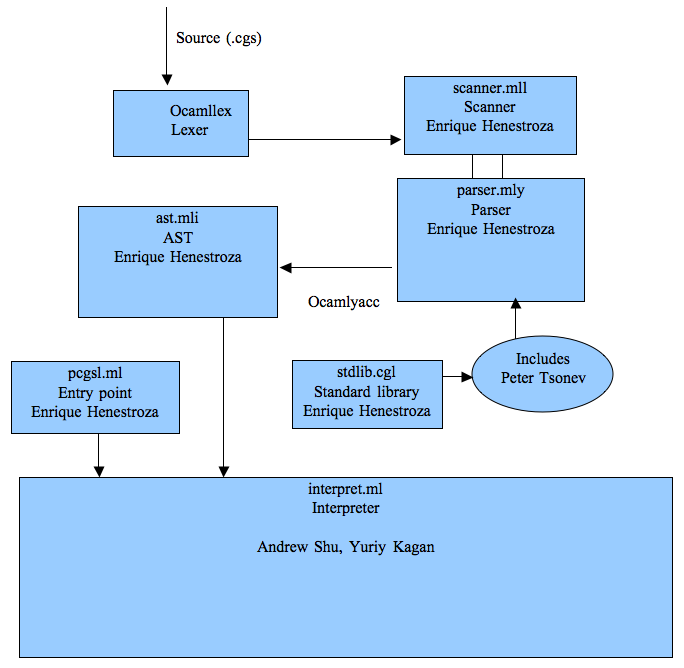
\includegraphics[scale=0.7]{picture1.png}

\end{document}


